In this chapter we train and validate the Behler-Parrinello
and DPMD on data obtained from molecular dynamics simulations
with classical potentials. We will focus on the Lennard-Jones
and Stillinger-Weber potentials, as these are likely the most
well-known and widely used potentials out there,
and are good candidates for benchmarking and testing
novel simulations. We will examine and compare the different
methods, and evaluate them relative to the empirical potentials
and each other. The methods will be evaluated on the metrics
of training and test error for both the energy and the forces,
the radial distribution function and some important mechanical properties.

\subsection{Input data}
The input data is a list of ASE Atoms objects or \textit{images},
which represent the state of the atoms at a given time.
The Lennard-Jones data is computed using the ASE "lj" calculator,
which is pure Python (e.g. slow) implementation of the Lennard-Jones potential.
The potential energy and forces is computed every timestep using this
calculator and the system is integrated forward in time using
the Velocity-Verlet algorithm. The simulation is performed in the NVE
ensemble with an initial velocity according to the Maxwell-Boltzmann
distribution with a temperature of 300K.
The initial state of the system is $2\times 2\times 2$
unit cells of the face-centered cubic crystal containing
4 atoms for a total of $4\times 2^3 = 32$ Argon atoms.
The system is integrated for a total of 1000 timesteps,
with the trajectory written to file every 10 timesteps.

\begin{figure}
    \centering
    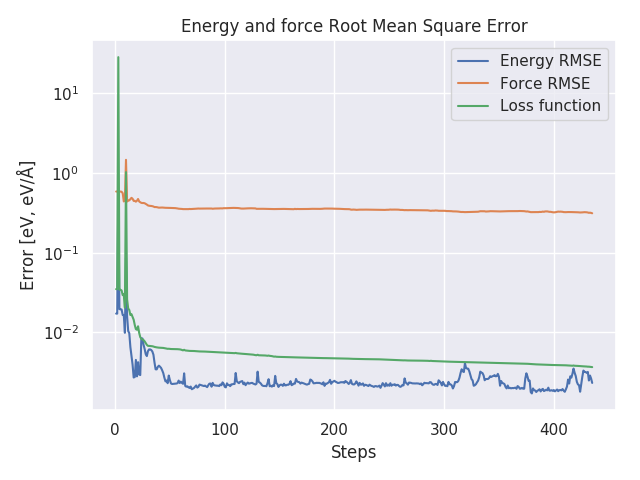
\includegraphics[width=\textwidth]{loss.png}
    \label{fig:}
    \caption{Text}
\end{figure}
